\documentclass{beamer}
\usepackage{amsmath}
\usepackage{amssymb}
\usepackage{tikz}
\usepackage{pgfplots}
\pgfplotsset{compat=1.17}

\usetheme{Madrid}
\usecolortheme{default}

\title{Diplomatic Treaty Negotiation Game}
\subtitle{A Parameterized Multi-Agent Bargaining Environment}
\author{Joie Zhang}
\date{January 7, 2026}

\begin{document}

\frame{\titlepage}

\begin{frame}{Overview}
\textbf{Goal}: Create a multi-agent negotiation environment where we can smoothly vary the level of competition vs cooperation

\vspace{0.5cm}

\textbf{Key Idea}: Agents negotiate over multiple issues simultaneously
\begin{itemize}
    \item Each agent has preferences about outcomes on each issue
    \item Each agent cares different amounts about different issues
    \item Issue structure determines if interests align or conflict
\end{itemize}

\vspace{0.5cm}

\textbf{Three orthogonal parameters} control competition level
\end{frame}

\begin{frame}{Basic Setup: The Negotiation Space}
\textbf{Components}:
\begin{itemize}
    \item $N$ agents (e.g., countries negotiating a treaty)
    \item $K$ issues to negotiate (e.g., trade, territory, military access)
    \item Agreement $A = [a_1, a_2, \ldots, a_K]$ where $a_k \in [0,1]$
\end{itemize}

\vspace{0.5cm}

\textbf{Example}: 2 countries, 3 issues
\begin{center}
\begin{tabular}{lcc}
\hline
Issue & Interpretation & Agreement Value \\
\hline
Tariff rate & 0\% to 100\% & $a_1 = 0.35$ (35\%) \\
Military base access & No to Full & $a_2 = 0.70$ (Partial) \\
Resource sharing & None to All & $a_3 = 0.50$ (Half) \\
\hline
\end{tabular}
\end{center}
\end{frame}

\begin{frame}{Agent Preferences: Two Components}
Each agent $i$ has:

\vspace{0.2cm}

\textbf{1. Position Preferences} $p_i = [p_{i1}, \ldots, p_{iK}]$
\begin{itemize}
    \item ``WHERE on each issue do I want the outcome to be?''
    \item $p_{ik} \in [0,1]$ is agent $i$'s ideal outcome on issue $k$
\end{itemize}

\vspace{0.3cm}

\textbf{2. Importance Weights} $w_i = [w_{i1}, \ldots, w_{iK}]$
\begin{itemize}
    \item ``HOW MUCH do I care about each issue?''
    \item $w_{ik} \geq 0$ and $\sum_k w_{ik} = 1$ (normalized)
\end{itemize}
\end{frame}

\begin{frame}{Agent Utility Function}
Agent $i$'s utility from agreement $A$:

\begin{equation*}
U_i(A) = \sum_{k=1}^{K} w_{ik} \cdot v_{ik}(a_k)
\end{equation*}

\vspace{0.3cm}

where $v_{ik}(a_k) = 1 - |p_{ik} - a_k|$ measures closeness to ideal

\vspace{0.5cm}

\textbf{Intuition}:
\begin{itemize}
    \item Get value from each issue proportional to how much you care ($w_{ik}$)
    \item Value is higher when outcome is closer to your ideal ($p_{ik}$)
    \item Perfect match: $a_k = p_{ik} \Rightarrow v_{ik} = 1$
    \item Maximum distance: $|a_k - p_{ik}| = 1 \Rightarrow v_{ik} = 0$
\end{itemize}
\end{frame}

\begin{frame}{Simple Example: 2 Agents, 2 Issues}
\begin{columns}
\column{0.5\textwidth}
\textbf{Agent 1}:
\begin{itemize}
    \item Positions: $p_1 = [0.3, 0.7]$
    \item Weights: $w_1 = [0.8, 0.2]$
    \item Cares most about issue 1
\end{itemize}

\vspace{0.5cm}

\textbf{Agent 2}:
\begin{itemize}
    \item Positions: $p_2 = [0.6, 0.4]$
    \item Weights: $w_2 = [0.3, 0.7]$
    \item Cares most about issue 2
\end{itemize}

\column{0.5\textwidth}
\textbf{Agreement}: $A = [0.4, 0.6]$

\vspace{0.3cm}

Agent 1 utility:
\begin{align*}
U_1(A) &= 0.8(1-|0.3-0.4|) \\
&\quad + 0.2(1-|0.7-0.6|) \\
&= 0.8(0.9) + 0.2(0.9) \\
&= 0.90
\end{align*}

Agent 2 utility:
\begin{align*}
U_2(A) &= 0.3(1-|0.6-0.4|) \\
&\quad + 0.7(1-|0.4-0.6|) \\
&= 0.3(0.8) + 0.7(0.8) \\
&= 0.80
\end{align*}
\end{columns}

\vspace{0.3cm}
\textbf{Note}: Different priorities allow both to do reasonably well!
\end{frame}

\begin{frame}{The Three Control Parameters}
\begin{center}
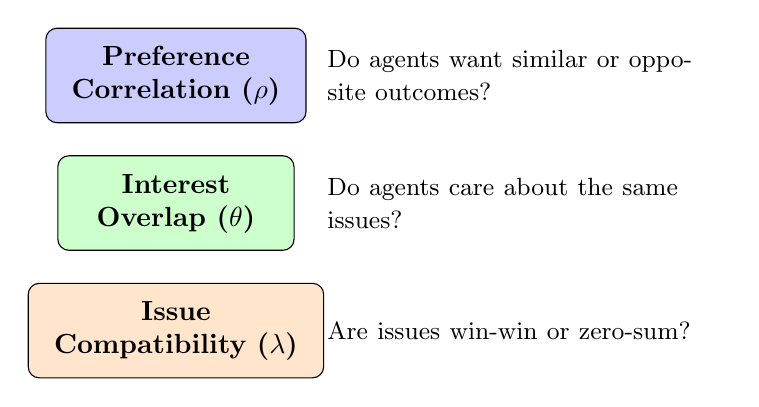
\begin{tikzpicture}[scale=0.9]
    % Parameter 1
    \node[draw, rectangle, rounded corners, fill=blue!20, minimum width=3cm, minimum height=1.2cm] at (0,3) 
        {\begin{tabular}{c} \textbf{Preference} \\ \textbf{Correlation ($\rho$)} \end{tabular}};
    \node[right, text width=5cm] at (2,3) {\small Do agents want similar or opposite outcomes?};
    
    % Parameter 2
    \node[draw, rectangle, rounded corners, fill=green!20, minimum width=3cm, minimum height=1.2cm] at (0,1.2) 
        {\begin{tabular}{c} \textbf{Interest} \\ \textbf{Overlap ($\theta$)} \end{tabular}};
    \node[right, text width=5cm] at (2,1.2) {\small Do agents care about the same issues?};
    
    % Parameter 3
    \node[draw, rectangle, rounded corners, fill=orange!20, minimum width=3cm, minimum height=1.2cm] at (0,-0.6) 
        {\begin{tabular}{c} \textbf{Issue} \\ \textbf{Compatibility ($\lambda$)} \end{tabular}};
    \node[right, text width=5cm] at (2,-0.6) {\small Are issues win-win or zero-sum?};
\end{tikzpicture}
\end{center}

\vspace{0.5cm}

These are \textbf{orthogonal}: you can independently control each one to explore different competitive scenarios
\end{frame}

\begin{frame}{Parameter 1: Preference Correlation ($\rho$)}
\textbf{Definition}: Correlation between agents' position preferences

\begin{equation*}
\rho \in [-1, 1]
\end{equation*}

\vspace{0.5cm}

\begin{columns}
\column{0.33\textwidth}
\centering
\textbf{$\rho = 1$}

Aligned

\vspace{0.2cm}

$p_1 \approx p_2$

\vspace{0.2cm}

Both want tariffs LOW or both want HIGH

\column{0.33\textwidth}
\centering
\textbf{$\rho = 0$}

Independent

\vspace{0.2cm}

No correlation

\vspace{0.2cm}

One wants tariffs at 30\%, other at 70\%

\column{0.33\textwidth}
\centering
\textbf{$\rho = -1$}

Opposed

\vspace{0.2cm}

$p_1 \approx 1 - p_2$

\vspace{0.2cm}

One wants HIGH, other wants LOW
\end{columns}

\vspace{0.5cm}

\textbf{Effect on competition}:
\begin{itemize}
    \item High $\rho$: Cooperative (want same things)
    \item Low/negative $\rho$: Competitive (want different things)
\end{itemize}
\end{frame}

\begin{frame}{Preference Correlation: Visual Example}
\textbf{3 Issues}: Trade, Security, Resources

\vspace{0.05cm}

\begin{center}
\textbf{High Correlation ($\rho = 1$)}: Agents want similar outcomes
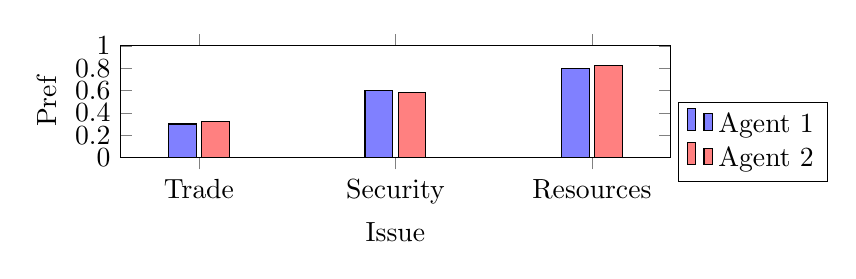
\begin{tikzpicture}
    \begin{axis}[
        width=8.57cm, height=3cm,
        ybar,
        bar width=10pt,
        xlabel={Issue},
        ylabel={Pref},
        symbolic x coords={Trade, Security, Resources},
        xtick=data,
        ymin=0, ymax=1,
        legend style={at={(1.15,0.5)}, anchor=north, legend columns=1},
        enlarge x limits=0.2
    ]
    
    % rho = 1 (aligned)
    \addplot[fill=blue!50] coordinates {(Trade,0.3) (Security,0.6) (Resources,0.8)};
    \addplot[fill=red!50] coordinates {(Trade,0.32) (Security,0.58) (Resources,0.82)};
    
    \legend{Agent 1, Agent 2}
    \end{axis}
\end{tikzpicture}
\end{center}

\vspace{0.01cm}

\begin{center}
\textbf{Negative Correlation ($\rho = -1$)}: Agents want opposite outcomes
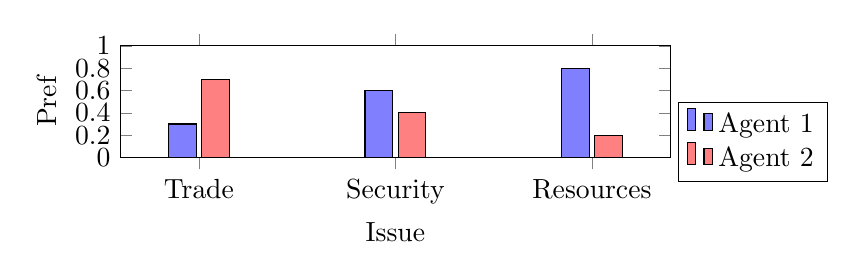
\begin{tikzpicture}
    \begin{axis}[
        width=8.57cm, height=3cm,
        ybar,
        bar width=10pt,
        xlabel={Issue},
        ylabel={Pref},
        symbolic x coords={Trade, Security, Resources},
        xtick=data,
        ymin=0, ymax=1,
        legend style={at={(1.15,0.5)}, anchor=north, legend columns=1},
        enlarge x limits=0.2
    ]
    
    % rho = -1 (opposed)
    \addplot[fill=blue!50] coordinates {(Trade,0.3) (Security,0.6) (Resources,0.8)};
    \addplot[fill=red!50] coordinates {(Trade,0.7) (Security,0.4) (Resources,0.2)};
    
    \legend{Agent 1, Agent 2}
    \end{axis}
\end{tikzpicture}
\end{center}
\end{frame}

\begin{frame}{Generating Preferences with Correlation $\rho$}
\textbf{Goal}: Create position preferences where agents' ideal outcomes are correlated

\vspace{0.3cm}

\textbf{Method}: Use multivariate normal distribution

For 2 agents, we want to generate correlated random variables:
\begin{equation*}
\begin{bmatrix} p_1 \\ p_2 \end{bmatrix} \sim \mathcal{N}\left(\mu, \Sigma\right)
\end{equation*}

where:
\begin{itemize}
    \item $\mu = \begin{bmatrix} 0.5 \\ 0.5 \end{bmatrix}$ is the mean vector (center of issue space)
    \item $\Sigma = \begin{bmatrix} \sigma^2 & \rho\sigma^2 \\ \rho\sigma^2 & \sigma^2 \end{bmatrix}$ is the covariance matrix
\end{itemize}

\vspace{0.3cm}

We generate this separately for each of the $K$ issues.
\end{frame}

\begin{frame}{Understanding the Notation}
\textbf{Breaking down the multivariate normal}:

\begin{equation*}
\begin{bmatrix} p_1 \\ p_2 \end{bmatrix} \sim \mathcal{N}\left(\begin{bmatrix} 0.5 \\ 0.5 \end{bmatrix}, \begin{bmatrix} \sigma^2 & \rho\sigma^2 \\ \rho\sigma^2 & \sigma^2 \end{bmatrix}\right)
\end{equation*}

\textbf{Parameters explained}:
\begin{itemize}
    \item $\mathcal{N}(\cdot, \cdot)$: Normal (Gaussian) distribution
    \item $\mu = 0.5$: Both agents' preferences centered at middle of issue space
    \item $\sigma^2$: Variance (how spread out preferences are). Try $\sigma = 0.25$
    \item $\rho$: Correlation coefficient $\in [-1, 1]$ - our control parameter!
\end{itemize}

\vspace{0.3cm}

\textbf{The covariance matrix $\Sigma$}:
\begin{itemize}
    \item Diagonal entries ($\sigma^2$): Variance of each agent's preferences
    \item Off-diagonal entries ($\rho\sigma^2$): Covariance between agents
    \item When $\rho = 0$: Off-diagonals are 0, agents independent
    \item When $\rho > 0$: Positive covariance, preferences move together
    \item When $\rho < 0$: Negative covariance, preferences move opposite
\end{itemize}
\end{frame}

\begin{frame}{How Correlation $\rho$ Works: Intuition}
\textbf{Think of it as joint sampling}:

\vspace{0.3cm}

\textbf{$\rho = 1$ (Perfect positive correlation)}:
\begin{itemize}
    \item If we randomly sample Agent 1's preference HIGH, then Agent 2's will also be HIGH
    \item If Agent 1 wants low tariffs, Agent 2 also wants low tariffs
    \item They move together perfectly
\end{itemize}

\vspace{0.3cm}

\textbf{$\rho = 0$ (No correlation)}:
\begin{itemize}
    \item Agent 1 and Agent 2's preferences are independent
    \item Knowing Agent 1 wants high tariffs tells you nothing about Agent 2
\end{itemize}

\vspace{0.3cm}

\textbf{$\rho = -1$ (Perfect negative correlation)}:
\begin{itemize}
    \item If Agent 1's preference is HIGH, then Agent 2's will be LOW
    \item If Agent 1 wants 80\% tariff, Agent 2 wants 20\% tariff
    \item They move in opposite directions
\end{itemize}
\end{frame}

\begin{frame}{Implementation Steps}
\textbf{Algorithm} (using Python/NumPy as example):

\begin{enumerate}
    \item Set parameters:
    \begin{itemize}
        \item Choose $\rho$ (your control parameter)
        \item Set $\sigma = 0.25$ (standard deviation)
        \item Set $\mu = 0.5$ (mean)
    \end{itemize}
    
    \item Construct covariance matrix:
    \begin{itemize}
        \item $\Sigma = \begin{bmatrix} 0.0625 & 0.0625\rho \\ 0.0625\rho & 0.0625 \end{bmatrix}$
    \end{itemize}
    
    \item For each issue $k = 1, \ldots, K$:
    \begin{itemize}
        \item Sample: $(p_{1k}, p_{2k}) \sim \mathcal{N}([0.5, 0.5], \Sigma)$
        \item Clip to valid range: $p_{ik} = \max(0, \min(1, p_{ik}))$
    \end{itemize}
    
    \item Result: Position preferences $p_1, p_2$ with correlation $\approx \rho$
\end{enumerate}

\vspace{0.3cm}

\textbf{For $N > 2$ agents}: Construct $N \times N$ covariance matrix with $\Sigma_{ij} = \rho\sigma^2$ for $i \neq j$
\end{frame}

\begin{frame}{Parameter 2: Interest Overlap ($\theta$)}
\textbf{Definition}: Cosine similarity between importance weight vectors

\begin{equation*}
\theta = \frac{w_1 \cdot w_2}{\|w_1\| \|w_2\|} = \sum_{k=1}^{K} w_{1k} w_{2k}
\end{equation*}

(Simplifies because weights are normalized: $\|w_i\| = 1$)

\vspace{0.5cm}

\begin{columns}
\column{0.5\textwidth}
\centering
\textbf{$\theta \approx 1$}

High overlap

\vspace{0.2cm}

Both care about \textbf{same} issues

\vspace{0.2cm}

$w_1 \approx w_2$

\vspace{0.2cm}

\textcolor{red}{Competitive!}

\column{0.5\textwidth}
\centering
\textbf{$\theta \approx 0$}

Low overlap

\vspace{0.2cm}

Care about \textbf{different} issues

\vspace{0.2cm}

$w_1 \perp w_2$

\vspace{0.2cm}

\textcolor{blue}{Trading potential!}
\end{columns}
\end{frame}

\begin{frame}{Interest Overlap: Visual Example}
\textbf{3 Issues}: Trade, Security, Resources

\vspace{0.3cm}

\begin{center}
\textbf{High Overlap} ($\theta = 0.95$) - Both prioritize Trade
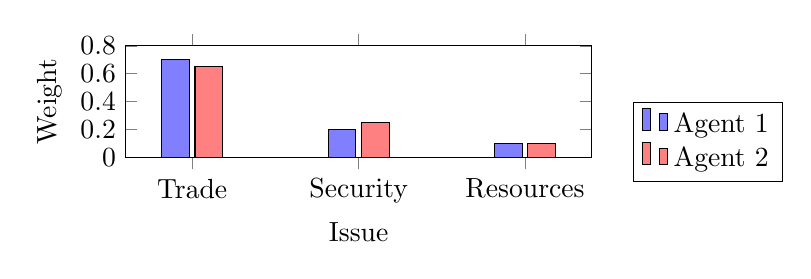
\begin{tikzpicture}
    \begin{axis}[
        width=7.5cm, height=3cm,
        ybar,
        bar width=10pt,
        xlabel={Issue},
        ylabel={Weight},
        symbolic x coords={Trade, Security, Resources},
        xtick=data,
        ymin=0, ymax=0.8,
        legend style={at={(1.25,0.5)}, anchor=north, legend columns=1},
        enlarge x limits=0.2
    ]
    
    \addplot[fill=blue!50] coordinates {(Trade,0.7) (Security,0.2) (Resources,0.1)};
    \addplot[fill=red!50] coordinates {(Trade,0.65) (Security,0.25) (Resources,0.1)};
    
    \legend{Agent 1, Agent 2}
    \end{axis}
\end{tikzpicture}
\end{center}

\begin{center}
\textbf{Low Overlap} ($\theta = 0.15$) - Agent 1 prio. Trade, Agent 2 prio. Security
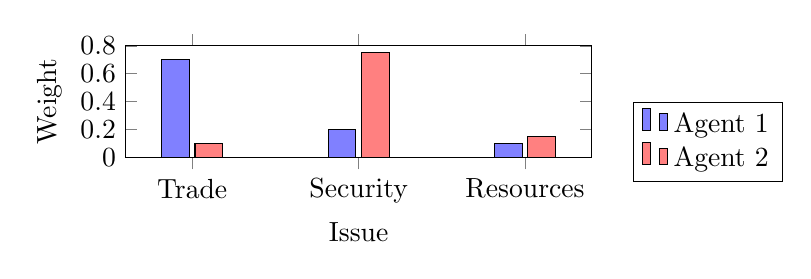
\begin{tikzpicture}
    \begin{axis}[
        width=7.5cm, height=3cm,
        ybar,
        bar width=10pt,
        xlabel={Issue},
        ylabel={Weight},
        symbolic x coords={Trade, Security, Resources},
        xtick=data,
        ymin=0, ymax=0.8,
        legend style={at={(1.25,0.5)}, anchor=north, legend columns=1},
        enlarge x limits=0.2
    ]
    
    \addplot[fill=blue!50] coordinates {(Trade,0.7) (Security,0.2) (Resources,0.1)};
    \addplot[fill=red!50] coordinates {(Trade,0.1) (Security,0.75) (Resources,0.15)};
    
    \legend{Agent 1, Agent 2}
    \end{axis}
\end{tikzpicture}
\end{center}
\end{frame}

\begin{frame}{Why Interest Overlap Matters}
\textbf{High Overlap} ($\theta \approx 1$): Competitive
\begin{itemize}
    \item Both agents fight over the \textbf{same issues}
    \item No room for tradeoffs: ``You care about trade? I care about trade too!''
    \item Zero-sum mentality: your gain on important issues is my loss
\end{itemize}

\vspace{0.5cm}

\textbf{Low Overlap} ($\theta \approx 0$): Integrative potential
\begin{itemize}
    \item Agents care about \textbf{different issues}
    \item Room for \textbf{logrolling}: ``I'll give you what you want on security if you give me what I want on trade''
    \item Classic integrative bargaining scenario
    \item Both can achieve high utility through smart tradeoffs
\end{itemize}

\vspace{0.3cm}

\textbf{Key insight}: Even if positions conflict ($\rho < 0$), low overlap ($\theta \approx 0$) enables cooperation!
\end{frame}

\begin{frame}{Generating Weights with Overlap $\theta$}
\textbf{Goal}: Create weight vectors $w_1, w_2$ with cosine similarity $\approx \theta_{\text{target}}$

\vspace{0.5cm}

\textbf{Algorithm}:
\begin{enumerate}
    \item Generate $w_1 \sim \text{Dirichlet}(\alpha, \alpha, \ldots, \alpha)$
    \begin{itemize}
        \item Dirichlet ensures positive weights that sum to 1
        \item Parameter $\alpha$ controls concentration (try $\alpha = 2$)
    \end{itemize}
    
    \item Generate candidate $w_2' \sim \text{Dirichlet}(\alpha, \alpha, \ldots, \alpha)$
    
    \item Mix: $w_2 = \theta_{\text{target}} \cdot w_1 + (1-\theta_{\text{target}}) \cdot w_2'$
    
    \item Renormalize: $w_2 \leftarrow w_2 / \sum_k w_{2k}$
    
    \item Verify: compute $\theta_{\text{actual}} = w_1 \cdot w_2$
\end{enumerate}

\vspace{0.3cm}

\textbf{Note}: Actual $\theta$ will be close but not exactly $\theta_{\text{target}}$ due to renormalization
\end{frame}

\begin{frame}{Parameter 3: Issue Compatibility ($\lambda$)}
\textbf{Definition}: Average compatibility across all issues

\begin{equation*}
\lambda = \frac{1}{K} \sum_{k=1}^{K} c_k \quad \text{where } c_k \in \{-1, 1\}
\end{equation*}

\vspace{0.3cm}

\textbf{Issue types}:
\begin{itemize}
    \item \textbf{Compatible} ($c_k = 1$): Win-win issue, both agents can do well
    \item \textbf{Conflicting} ($c_k = -1$): Zero-sum issue, one's gain is other's loss
\end{itemize}

\vspace{0.5cm}

\begin{columns}
\column{0.33\textwidth}
\centering
\textbf{$\lambda = 1$}

All compatible

Fully integrative

\column{0.33\textwidth}
\centering
\textbf{$\lambda = 0$}

Mixed issues

Half and half

\column{0.33\textwidth}
\centering
\textbf{$\lambda = -1$}

All conflicting

Fully distributive
\end{columns}
\end{frame}

\begin{frame}{Compatible Issues (Win-Win)}
\textbf{Characteristic}: Both agents can achieve high utility simultaneously

\vspace{0.3cm}

\textbf{Example - Environmental Protection}:
\begin{itemize}
    \item Agent 1 position: $p_{1k} = 0.7$ (strong protection)
    \item Agent 2 position: $p_{2k} = 0.6$ (strong protection)
    \item Agreement at $a_k = 0.65$ makes both happy!
    \item $v_{1k}(0.65) = 1 - |0.7 - 0.65| = 0.95$
    \item $v_{2k}(0.65) = 1 - |0.6 - 0.65| = 0.95$
\end{itemize}

\vspace{0.3cm}

\textbf{Key property}: Preferences are aligned or have a ``sweet spot''

\vspace{0.3cm}

\textbf{Implementation}: Generate positions with positive correlation on compatible issues, or define utility function with shared optimal region
\end{frame}

\begin{frame}{Conflicting Issues (Zero-Sum)}
\textbf{Characteristic}: One agent's gain is exactly the other's loss

\vspace{0.3cm}

\textbf{Example - Territory Division}:
\begin{itemize}
    \item Issue represents \% of disputed territory to Agent 1
    \item Agent 1 utility: $v_{1k}(a_k) = a_k$ (wants more)
    \item Agent 2 utility: $v_{2k}(a_k) = 1 - a_k$ (wants Agent 1 to get less)
    \item Notice: $v_{1k}(a_k) + v_{2k}(a_k) = 1$ (constant sum)
\end{itemize}

\vspace{0.3cm}

\textbf{Key property}: $p_{2k} = 1 - p_{1k}$ (perfectly opposed)

\vspace{0.3cm}

\textbf{Implementation}:
\begin{itemize}
    \item Set opposing preferences: $p_{2k} = 1 - p_{1k}$
    \item Use linear utility: $v_{1k}(a_k) = a_k$, $v_{2k}(a_k) = 1-a_k$
\end{itemize}
\end{frame}

\begin{frame}{Generating Issues with Compatibility $\lambda$}
\textbf{Goal}: Create $K$ issues where average compatibility = $\lambda$

\vspace{0.5cm}

\textbf{Algorithm}:
\begin{enumerate}
    \item Compute probability: $p = \frac{\lambda + 1}{2}$
    \begin{itemize}
        \item $\lambda = 1 \Rightarrow p = 1$ (all compatible)
        \item $\lambda = 0 \Rightarrow p = 0.5$ (50-50 mix)
        \item $\lambda = -1 \Rightarrow p = 0$ (all conflicting)
    \end{itemize}
    
    \item For each issue $k = 1, \ldots, K$:
    \begin{itemize}
        \item Sample $u \sim \text{Uniform}(0,1)$
        \item If $u < p$: set $c_k = 1$ (compatible issue)
        \item Otherwise: set $c_k = -1$ (conflicting issue)
    \end{itemize}
    
    \item Generate preferences/utilities according to issue type
\end{enumerate}

\vspace{0.3cm}

\textbf{Result}: Expected value $\mathbb{E}[c_k] = p \cdot 1 + (1-p) \cdot (-1) = \lambda$ (check!)
\end{frame}

\begin{frame}{Putting It All Together: Example Scenario}
\textbf{Moderate Competition Setup}:
\begin{itemize}
    \item $\rho = -0.3$: Somewhat opposing preferences
    \item $\theta = 0.4$: Moderate priority overlap (some trading potential)
    \item $\lambda = 0.2$: Mostly conflicting issues (60\% conflicting, 40\% compatible)
\end{itemize}

\vspace{0.5cm}

\textbf{Generated Instance} (2 agents, 5 issues):

\begin{center}
\small
\begin{tabular}{lccccc}
\hline
 & \textbf{Issue 1} & \textbf{Issue 2} & \textbf{Issue 3} & \textbf{Issue 4} & \textbf{Issue 5} \\
\hline
Type & Conflict & Conflict & Compatible & Conflict & Compatible \\
$c_k$ & -1 & -1 & +1 & -1 & +1 \\
\hline
$p_1$ & 0.65 & 0.30 & 0.55 & 0.75 & 0.40 \\
$p_2$ & 0.35 & 0.80 & 0.50 & 0.20 & 0.45 \\
\hline
$w_1$ & 0.40 & 0.15 & 0.10 & 0.25 & 0.10 \\
$w_2$ & 0.20 & 0.35 & 0.15 & 0.20 & 0.10 \\
\hline
\end{tabular}
\end{center}

\vspace{0.3cm}

\textbf{Observation}: Agent 1 prioritizes Issues 1 \& 4; Agent 2 prioritizes Issue 2 → logrolling possible!
\end{frame}

\begin{frame}{Competition Level Summary}
\begin{center}
\begin{tabular}{lccc}
\hline
\textbf{Parameter} & \textbf{Cooperative} & \textbf{Neutral} & \textbf{Competitive} \\
\hline
$\rho$ (Preferences) & $+1$ & $0$ & $-1$ \\
 & Aligned & Uncorrelated & Opposed \\
\hline
$\theta$ (Priorities) & $0$ & $0.5$ & $1$ \\
 & Different & Mixed & Same \\
\hline
$\lambda$ (Issues) & $+1$ & $0$ & $-1$ \\
 & Win-win & Mixed & Zero-sum \\
\hline
\end{tabular}
\end{center}

\vspace{0.5cm}

\textbf{Pure Cooperation}: $(\rho, \theta, \lambda) = (1, 0, 1)$
\begin{itemize}
    \item Agents want same outcomes, care about different things, all issues win-win
\end{itemize}

\vspace{0.3cm}

\textbf{Pure Competition}: $(\rho, \theta, \lambda) = (-1, 1, -1)$
\begin{itemize}
    \item Agents want opposite outcomes, care about same things, all issues zero-sum
\end{itemize}
\end{frame}

\begin{frame}{Why These Parameters Are Orthogonal}
\textbf{Independence}: You can vary each parameter without affecting the others

\vspace{0.5cm}

\begin{itemize}
    \item \textbf{$\rho$ vs $\theta$}: Position correlation is separate from weight overlap
    \begin{itemize}
        \item Can have aligned positions ($\rho=1$) but different priorities ($\theta=0$)
        \item Can have opposed positions ($\rho=-1$) but same priorities ($\theta=1$)
    \end{itemize}
    
    \vspace{0.3cm}
    
    \item \textbf{$\rho$ vs $\lambda$}: Position correlation is separate from issue structure
    \begin{itemize}
        \item Can have aligned positions on zero-sum issues
        \item Can have opposed positions on win-win issues
    \end{itemize}
    
    \vspace{0.3cm}
    
    \item \textbf{$\theta$ vs $\lambda$}: Weight overlap is separate from issue structure
    \begin{itemize}
        \item Can have same priorities ($\theta=1$) on win-win issues ($\lambda=1$)
        \item Can have different priorities ($\theta=0$) on zero-sum issues ($\lambda=-1$)
    \end{itemize}
\end{itemize}

\vspace{0.3cm}

This allows systematic exploration of the cooperation-competition space!
\end{frame}

\begin{frame}{Measuring Negotiation Outcomes}
\textbf{Social Welfare}: Total utility across agents
\begin{equation*}
SW(A) = \sum_{i=1}^{N} U_i(A)
\end{equation*}

\vspace{0.3cm}

\textbf{Pareto Efficiency}: No other agreement makes someone better off without making someone worse off

\vspace{0.3cm}

\textbf{Utilitarian Distance}: How far from optimal social welfare?
\begin{equation*}
D_U = \frac{SW^* - SW(A)}{SW^*} \in [0,1]
\end{equation*}
$D_U = 0$: Optimal, $D_U = 1$: Worst possible

\vspace{0.3cm}

\textbf{Expected behavior}:
\begin{itemize}
    \item Cooperative settings: Low $D_U$ (near Pareto frontier)
    \item Competitive settings: High $D_U$ (inefficient outcomes)
\end{itemize}
\end{frame}

\begin{frame}{Using This Environment}
\textbf{Research questions you can explore}:

\begin{enumerate}
    \item How do different negotiation protocols perform across competition levels?
    
    \item Do agents learn to identify and exploit integrative potential (low $\theta$)?
    
    \item How does increasing $N$ (number of agents) affect cooperation?
    
    \item Can agents learn to truthfully reveal preferences vs strategically misrepresent?
    
    \item What communication structures help most in competitive settings?
\end{enumerate}

\vspace{0.5cm}

\textbf{Advantages}:
\begin{itemize}
    \item Richer strategic space (positions + priorities + issue structure)
    \item Multiple dimensions of competition (not just single cosine similarity)
    \item Captures realistic negotiation dynamics (logrolling, tradeoffs)
\end{itemize}
\end{frame}

\begin{frame}{Summary: Quick Reference}
\textbf{Three Control Parameters}:

\begin{enumerate}
    \item \textbf{$\rho \in [-1,1]$}: Preference correlation
    \begin{itemize}
        \item Do agents want similar ($\rho=1$) or opposite ($\rho=-1$) outcomes?
    \end{itemize}
    
    \item \textbf{$\theta \in [0,1]$}: Interest overlap (cosine similarity of weights)
    \begin{itemize}
        \item Do agents care about same ($\theta=1$) or different ($\theta=0$) issues?
    \end{itemize}
    
    \item \textbf{$\lambda \in [-1,1]$}: Issue compatibility (mean of $c_k$)
    \begin{itemize}
        \item Are issues win-win ($\lambda=1$) or zero-sum ($\lambda=-1$)?
    \end{itemize}
\end{enumerate}

\vspace{0.5cm}

\textbf{Key Formula}:
\begin{equation*}
U_i(A) = \sum_{k=1}^{K} w_{ik} \cdot (1 - |p_{ik} - a_k|)
\end{equation*}

\textbf{Remember}: These parameters are orthogonal $\rightarrow$ systematic exploration of cooperation-competition space
\end{frame}

\begin{frame}{Wait... Do We Really Need 3 Parameters?}
\textbf{You're right to question this!} Let me make the case for why 3 is justified:

\vspace{0.5cm}

\textbf{The Core Problem}: 
\begin{itemize}
    \item Our item allocation game has 1 parameter (cosine similarity)
    \item It smoothly varies competition, but collapses multiple aspects into one dimension
    \item Real negotiations have multiple \textit{types} of conflict and cooperation
\end{itemize}

\vspace{0.5cm}

\textbf{Why 3 parameters capture fundamentally different things}:
\begin{enumerate}
    \item \textbf{$\rho$}: ``Do we want the same things?'' (preference alignment)
    \item \textbf{$\theta$}: ``Do we care about the same things?'' (priority alignment)
    \item \textbf{$\lambda$}: ``Can we both win?'' (structural possibility)
\end{enumerate}

These are not just ``more dimensions'' - they're qualitatively different sources of conflict!
\end{frame}

\begin{frame}{The Problem with Collapsing to 1 Parameter}
\textbf{Example}: Consider two scenarios with ``medium competition''

\vspace{0.3cm}

\textbf{Scenario A}: Labor-Management Negotiation
\begin{itemize}
    \item \textit{Opposing preferences} ($\rho = -0.8$): Workers want higher wages, management wants lower
    \item \textit{BUT different priorities} ($\theta = 0.2$): Workers care most about wages, management cares most about work rules
    \item \textit{Mixed issues} ($\lambda = 0$): Some zero-sum (wage level), some integrative (flexible scheduling)
    \item \textbf{Outcome}: Hard bargaining, but room for creative tradeoffs
\end{itemize}

\vspace{0.3cm}

\textbf{Scenario B}: Two Tech Companies Standardizing
\begin{itemize}
    \item \textit{Similar preferences} ($\rho = 0.7$): Both want similar technical standards
    \item \textit{Same priorities} ($\theta = 0.9$): Both care about same features
    \item \textit{Zero-sum} ($\lambda = -0.8$): Each wants their own standard adopted (network effects)
    \item \textbf{Outcome}: Easy to agree on what, but problem on whose
\end{itemize}

\end{frame}

\begin{frame}{What Each Parameter Enables (That Others Don't)}
\begin{center}
\small
\begin{tabular}{p{2cm}p{4cm}p{4cm}}
\hline
\textbf{Parameter} & \textbf{Unique Insight} & \textbf{Lost if Removed} \\
\hline
$\rho$ & Preference conflict vs alignment & Can't distinguish ``we both want peace'' from ``I want war, you want peace'' \\
\hline
$\theta$ & Logrolling potential & Can't capture ``I'll give you X if you give me Y'' dynamics \\
\hline
$\lambda$ & Structural possibility of win-win & Can't model ``no matter what we do, only one can win'' vs ``we can both get 80\%'' \\
\hline
\end{tabular}
\end{center}

\vspace{0.5cm}

\textbf{Research value}:
\begin{itemize}
    \item Can agents \textit{discover} that low $\theta$ enables trading?
    \item Do agents behave differently when $\lambda < 0$ (zero-sum) vs $\lambda > 0$ (integrative)?
    \item Does high $\rho$ lead to faster agreement even if $\lambda = -1$?
\end{itemize}
\end{frame}

\begin{frame}{Simplified Version 1: Two Parameters}
\textbf{If you must reduce to 2, here's the best approach}:

\vspace{0.5cm}

\textbf{Keep}: $\rho$ (preference correlation) and $\theta$ (interest overlap)

\textbf{Fix}: $\lambda = 0$ (50-50 mix of compatible and conflicting issues)

\vspace{0.5cm}

\textbf{Why this works}:
\begin{itemize}
    \item $\rho$ and $\theta$ are the most behaviorally distinct
    \item $\rho$ controls \textit{what} agents want (positions)
    \item $\theta$ controls \textit{how much} they care (priorities)
    \item Mixed issue types ($\lambda = 0$) provides enough structure variety
    \item Still captures the key insight: integrative potential from different priorities
\end{itemize}

\vspace{0.3cm}

\textbf{Trade-off}: 
\begin{itemize}
    \item Lose ability to study pure zero-sum vs pure integrative scenarios
    \item But retain most of the strategic complexity
\end{itemize}
\end{frame}

\begin{frame}{Simplified Version 2: One Parameter}
\textbf{If you really want just 1 parameter for direct comparison to your current game}:

\vspace{0.5cm}

\textbf{Option A - Competition Index} $c \in [0,1]$:
\begin{align*}
\rho &= 1 - 2c \quad \text{(goes from 1 to -1)} \\
\theta &= c \quad \text{(goes from 0 to 1)} \\
\lambda &= 1 - 2c \quad \text{(goes from 1 to -1)}
\end{align*}

\begin{itemize}
    \item $c = 0$: Pure cooperation ($\rho=1, \theta=0, \lambda=1$)
    \item $c = 1$: Pure competition ($\rho=-1, \theta=1, \lambda=-1$)
\end{itemize}

\vspace{0.3cm}

\textbf{Option B - Keep only $\theta$} (like your cosine similarity):
\begin{itemize}
    \item Fix: $\rho = 0$ (uncorrelated preferences)
    \item Fix: $\lambda = 0$ (mixed issues)
    \item Vary: $\theta \in [0,1]$ (interest overlap)
    \item \textbf{Advantage}: Focuses on the integrative bargaining insight
    \item \textbf{Limitation}: Misses preference alignment effects
\end{itemize}
\end{frame}

\begin{frame}{My Recommendation: Start with 2, Scale to 3}
\textbf{Practical approach for your benchmark}:

\vspace{0.5cm}

\textbf{Phase 1 - Core Benchmark}: Use $\rho$ and $\theta$ (fix $\lambda = 0$)
\begin{itemize}
    \item Easier to explain and visualize (2D grid of difficulty)
    \item Captures the key multi-issue dynamics
    \item Directly comparable to your item allocation game
    \item Grid: $\rho \in \{-1, -0.5, 0, 0.5, 1\}$, $\theta \in \{0, 0.25, 0.5, 0.75, 1\}$
    \item That's 25 difficulty levels - plenty for benchmarking!
\end{itemize}

\vspace{0.5cm}

\textbf{Phase 2 - Extended Analysis}: Add $\lambda$ for deeper studies
\begin{itemize}
    \item Once baseline results are established
    \item Investigate: ``Do agents behave differently on pure zero-sum vs integrative?''
    \item Allows comparison with game theory predictions (Nash equilibrium vs Pareto)
\end{itemize}

\vspace{0.3cm}

\textbf{This gives you}: Simple core + extensibility for research questions
\end{frame}

\begin{frame}{Comparison to Your Item Allocation Game}
\begin{center}
\begin{tabular}{lcc}
\hline
\textbf{Aspect} & \textbf{Item Allocation} & \textbf{Diplomatic Treaty} \\
\hline
Control parameters & 1 (cosine sim) & 2-3 ($\rho, \theta, \lambda$) \\
Strategic space & Utility vectors & Positions + Weights \\
Cooperation type & Preference alignment & Multiple types \\
Interpretability & Very clear & Slightly more complex \\
Real-world analog & Resource allocation & Multi-issue bargaining \\
Scalability & Easy to $N > 2$ & Easy to $N > 2$ \\
Logrolling & Implicit & Explicit \\
\hline
\end{tabular}
\end{center}

\vspace{0.5cm}

\textbf{Bottom line}:
\begin{itemize}
    \item Item allocation: Great for clean, simple benchmark
    \item Diplomatic treaty (2-param): Better for realistic multi-issue dynamics
    \item Diplomatic treaty (3-param): Best for comprehensive research program
\end{itemize}

\textbf{Use both!} Different environments test different capabilities.
\end{frame}

\end{document}